COMPUTING

Line 73:

%, some older calculations from 2011 by Fujitsu put the figure at about 50\% for a specific model~\cite{Bordage}).

Line 87:

%CERN encourages knowledge transfer of technological advances,  %https://hse.cern/environment-report-2019-2020/knowledge-transfer

Line 93:

%Moreover, such designated efforts may allow new symbiotic collaborations on software outside the field. \ACR\ software components could find use in industry and vice versa, and the community can adopt software elements from outside rather than reinventing them.  Truly sustainable software development (in all senses) will give \ACR\ software developers an important skill essential to careers in the industry.
%They should, in general, follow 

Line 95:

%TODO: This effort was a collaboration between computer scientists and physicists. It is not yet documented (and released), so need to double check for wording 

Line 102:

%%Note: below is a further examples from ATLAS
%\textcolor{Pythonblue}{To do.}
%NOTE: THIS IS COPIED BITS FROM THE ACTUAL PAPER
%In multi-process (MP) parallelism, workers are forked from the primary process at a pre-configured stage during execution (\eg before or after the first event is processed). Following the forking, all worker processes share memory allocated in the primary process but otherwise run in parallel, independent of each other. As such, each worker also has its own unique memory space and produces its own outputs, which need to be merged later via a post-processing step.
%Multi-thread (MT) parallelism is significantly more challenging to develop. Here, there is no explicit forking of worker processes from the primary. Rather, threads are spawned and assigned some work (\eg execute an algorithm). There is a single pool of heap memory that is shared across all threads. This means that various difficulties must be overcome: multiple threads cannot write to the same memory at the same time; threads must not attempt to read memory that is actively being written to; and algorithms must be scheduled such that all input is fully available before they run. Because of these difficulties, writing MT-safe code can be demanding. However, the performance benefit from using a single pool of memory for all threads can be significant.

%The tests are run on a machine with an Intel®Xeon®CPU E5-2630 v3 at 2.40 GHz (16 cores, and with SMT disabled). The machine has 126 GB of available memory. Memory is measured by the proportional set size, and time by the wall clock processing time. For MP and MT tests, the number of events to be processed concurrently is set to the number of available threads. In some comparisons, the results from several serial (single thread, single process) reconstruction jobs are also shown. In these cases, the jobs do not interact with one another except through system-wide resource contention.

Line 103:

% Hannah Wakeling : With CERN's knowledge transfer policy, an environmental monitoring spin-off company 'PlanetWatch' has a license agreement for the CERN Control and Monitoring Platform, C2MON, to "deploy dense, real-time air quality monitoring networks in cities in a fast and cost-effective way". %https://hse.cern/environment-report-2019-2020/knowledge-transfer

Line 108:

% \begin{to_do}
% Infrastructure section, to include cloud computing.\\
% % Would cloud computing come under hardware (as it is remote?) or infrastructure? I vote infrastructure. 
% % Cloud jobs should be run in low carbon regions. % https://arxiv.org/pdf/2002.05651.pdf
% \end{to_do}

Line 182:

%The PUE, defined as total facility power/IT equipment energy, is a measure of a data centre's `overhead' energy costs, and a standard metric by which their energy efficiencies can be compared.  For reference, currently operational data centres have PUEs ranging from 1.2--1.5, with the average around 1.4. 

ENERGY

Line 51:

% We discuss the viability of different sources of sustainable energy below. 

% In addition, the sustainability of nuclear power is a question of much debate.

Line 54:

% This challenge must be overcome by a combination of transitioning to sustainable sources of energy, and energy-saving measures, both of which are discussed below.


% Global primary energy consumption in 2019 was approximately 160,000~TWh (equivalent to an average power consumption of 18,000~GW), around 80\,\% of which comes from \CdO-emitting fossil fuels~\cite{OWDfuels}. Moreover demand is rising, primarily due to the growth and industrialization of emerging countries.  A reduction to net zero emissions by 2040, as stipulated in the Paris Agreement, will create a huge global energy gap, as shown in \fref{fig:ene-gap}, and require the world to undergo a rapid transition to zero-carbon energy sources.   If this energy gap is not filled in the coming two decades, not just modern comforts, but also essential functions of our society, including food production for the estimated 9 billion people living on this planet, will be jeopardised.

%The requirement to reduce those to zero until 2040 creates a huge global energy gap as shown in . Fossil fuels today correspond to 15,000~GW of energy production. Adding the additional energy demand of emerging countries, using a naïve linear extrapolation, adds another 7,000~GW to the energy gap in 2040.

% The short time-frame for this transition will likely result in energy becoming scarce and expensive in the coming decades, making sourcing sustainable energy, and energy saving and recuperation in experiment and infrastructure design a priority for experimental \ACR, and experimental HEP in particular.  Ignoring these considerations will likely impact our capability of conducting energy-intensive experiments and data analysis in basic research, due to stringent energy restrictions. Today's planning of future experiments will be irrelevant if the implications of climate change are not taken into account.

% The options to cover the remaining energy needs are nuclear power and sustainable energy sources, such as solar or wind. We argue that, due to the timescale for construction of new plants, nuclear power cannot solve the energy gap (see \csref{cs:nuclear_gap}). For most \ACR\ institutions, such a rapid shift will only be possible through large-scale importation of sustainable energy.  World-leading research centres like CERN are uniquely placed to implement such schemes, with their history of cooperation across political and ideological boundaries.  We provide a concrete case study \csref{case:desert} of importing inexpensive renewable power from the sun-belts of North Africa to scientific institutions on the European power grid.

% Additional measures to reduce the \CdO\ content of the atmosphere have been proposed to offset some carbon consumption. These can be achieved either through biomass production with black carbon sequestration, or through \CdO\ sequestration from the atmosphere and exhaust gases.
% However, these are less promising than reducing emissions and mostly lie outside of the purview of the \ACR\ community.

%\footnote{IPPC, The Physical Science Basis Summary for Policymakers, Climate Change 2021, Summary for Policymakers; \url{https://www.ipcc.ch/site/assets/uploads/sites/2/2019/05/SR15\_SPM\_version\_report\_LR.png}}.

Line 61:

% \begin{itemize}
%         \item Take energy profiles into account when deciding on office appliances (\eg fridge, coffee machine).
%         \item Implement monitoring to understand energy usage and consider improvements.
%         \item Ensure that energy consumption is a central consideration in the design process for new experiments.
%     \end{itemize}

Line 69:

       %\item `Game-ify' decreasing energy use with \eg monthly cross-departmental competitions.

Line 78:

% \subsection{\ACR\ Energy Usage}

Line 93:

% A concrete case study of importing inexpensive renewable power from the sun-belts of North Africa to scientific institutions on the European power grid can be found in \csref{case:desert}. 

Line 101:

 %Costs for wind energy production elsewhere are too high to be competitive except for very small localized spots, \eg in South Norway or the Mediterranean}. 

 Line 103:

 %making wind energy more than a factor of 4 less efficient than to solar energy. 

 Line 125:

 % The exact role of nuclear power in a sustainable energy transition is therefore much disputed.

 Line 126:

 %\textcolor{red}{More recently, the increase in extreme heat has caused additional issues for the cooling of nuclear power plants~\cite{GuardianEDFNuclear}.}

Line 129:

% The exact role of nuclear power in a sustainable energy transition is much disputed.  

% An energy transition within the tight time frame of the Paris Agreement can involve none of the new nuclear technologies --- including nuclear fusion --- as they are not mature enough for global roll-out.  According to the \acrshort{iaea}, nuclear reactors have a median construction time of 93 months~\cite{IAEANuclear}, not including planning and permissions. Thus a more damning argument against nuclear energy is the unfeasibly large number of nuclear power stations one would need to construct in a short time-scale in order to cover global energy needs. This is discussed in the case study~\csref{case:nuclear} below.

Line 139:

% Promising methods to fill this gap are summarized in \tref{tab:EnergyStorage}, excerpted (with appended information) from~\cite{}.

Line 140:

% \begin{table}[h!]
% \centering

% \ra{1.05}
% {\scriptsize
% \begin{tabular}{>{\kern-\tabcolsep}p{2cm}wp{4cm}ccc<{\kern-\tabcolsep}}
% \toprule
% \textbf{Stored energy} & \textbf{Technology} & \textbf{Market readiness} & \textbf{Max size (MW)} & \textbf{Average RTE (\%)}\\
% \multirow{5}{*}{\parbox[t]{20mm}{Mechanical\\(potential/kinetic)}} & Novel pumped hydro (underground reservoir)& Commercial& 10 - 100 & 50-80 \\
%  & Gravity-based (lifting a weight) & Pilot & 20-1000 & 70-90 \\
%  & Compressed air & Commercial & 200-500 & 40-70 \\
%  & Liquid air & Pilot & 50-100 & 40-70 \\
%  & Liquid \CdO\ & Pilot & 10-500 & 70-80\\
%  \midrule
%  \multirow{2}{*}{\parbox[t]{20mm}{Thermal\\(in solid/liquid)}} & Sensible heat (e.g. in molten salts, rock, concrete) & Pilot & 10-500 & 55-90 \\
%  & Latent heat (e.g. in aluminium alloy) & Commercial & 10-100 & 20-50 \\
%  \midrule
% \end{tabular}
% }
% \end{table}
% \begin{to_do}
% Discussion of various forms of energy storage: batteries versus hydroelectric or mechanical storage, as well as the ways energy grids can be managed to deal with the changes in relative production from different renewables.\\
% \end{to_do}



% Recent drops in cost for lithium-ion batteries, which have decreased by a factor of 40 in the last 30 years~\cite{Ziegler_2020}, and solar panels (see \fref{fig:ene-costs}), have unlocked the potential for decentralised, economically viable, sustainable power production. This would help reduce foreign energy import dependencies, particularly of coal, gas, oil and uranium. 

Line 144:

%According to Ref.~\cite{MacKayhotair}, which reviews options for the energy transition with a specific focus on the United Kingdom, ``Any plan that doesn't make heavy use of nuclear power or `clean coal' has to make up the energy balance using renewable power bought in from other countries''.

Line 145:

% \begin{to_do}
% SLAC example on moving hydro power.\\
% \end{to_do}

Line 172:

% \paragraph{Importing sustainable energy}

% The uneven geographical distribution of sources of renewable energy naturally begs the question of whether large-scale importing of renewable energy could be a cost-effective way of closing the energy gap.  According to Ref.~\cite{MacKayhotair}, which reviews options for energy transition with a specific focus on the United Kingdom, ``Any plan that doesn't make heavy use of nuclear power or `clean coal' has to make up the energy balance using renewable power bought in from other countries''.
% While the resource is already more than 10 years old, its main points are still relevant. The author is about a factor of 4 less optimistic about the wind energy potential compared to the above cited recent EU report, which possibly reflects an increase in efficiency. However, even in the EU publication, the fraction of agricultural land deemed acceptable to be ceded to energy production is very small: only 4.4\,\%. This number illustrates that any of the renewable energy solutions are highly constrained by population density and alternative uses of land. Contributions from energy sources other than wind, water or solar are relatively small (\eg tidal power or waste incineration).

% Technical options to transport electricity over long distances have improved significantly in the last decades. In South America and China, projects to transport electricity over more than 2,000~km by Ultra High Voltage Direct Current (\acrshort{uhvdc}) lines are already operational~\cite{Champion}.%.  The evolution of subsea High Voltage Direct Current (\acrshort{hvdc}) cable technology is evident in the recently-inaugurated NordLink connection between Germany and Norway, consisting of 516~km of subsea HVDC cable.

% This technological progress opens up an alternative to the traditional import of chemical energy: direct import of renewable electricity from Northern Africa~\cite{Dueren,Dueren+2011+263+275}. An excellent potential for electricity generation by solar and wind power, large unused tracts of land, and existing energy trade partnerships for fossil fuels make North African countries ideal export partners for procuring electricity from sustainable sources.  HEP has a record of successful collaboration between nations and could thus be an important player in making this happen.  Hence, importing renewable energy should be considered as part of a catalogue of solutions to cover our future energy needs.  One possible scenario for the import of solar energy is detailed in the \csref{case:desert} below. 

% While the import of energy is a promising solution on the technical and economic level, constructing wind or solar farms, \eg in the sun belts of Africa to then export the power to Europe involves geopolitical and social considerations. Resource and person-power extraction from Africa to the benefit of Europe and America has a long and damnable colonial history. Therefore, it is of utmost importance to make fair power trade agreements between the continents that ensure strong integration into local communities and include the local population in the planning and implementation of such projects and related infrastructure. In this way, a win-win situation for all stakeholders should be ensured. Moreover, well planned cooperation has the potential to act in a geopolitically stabilizing way in line with the 16th and 17th UN SDGs.

Line 174:

% in governance, bringing people from different countries, continents and cultures together to focus all their effort and money towards a few most important scientific questions that they agreed on. Beyond science, 

Line 175:

%, and is deserving of continued funding.

Line 202:

% \paragraph{Nuclear power}




%%%%%

% \begin{figure}[!ht]
%      \centering
%      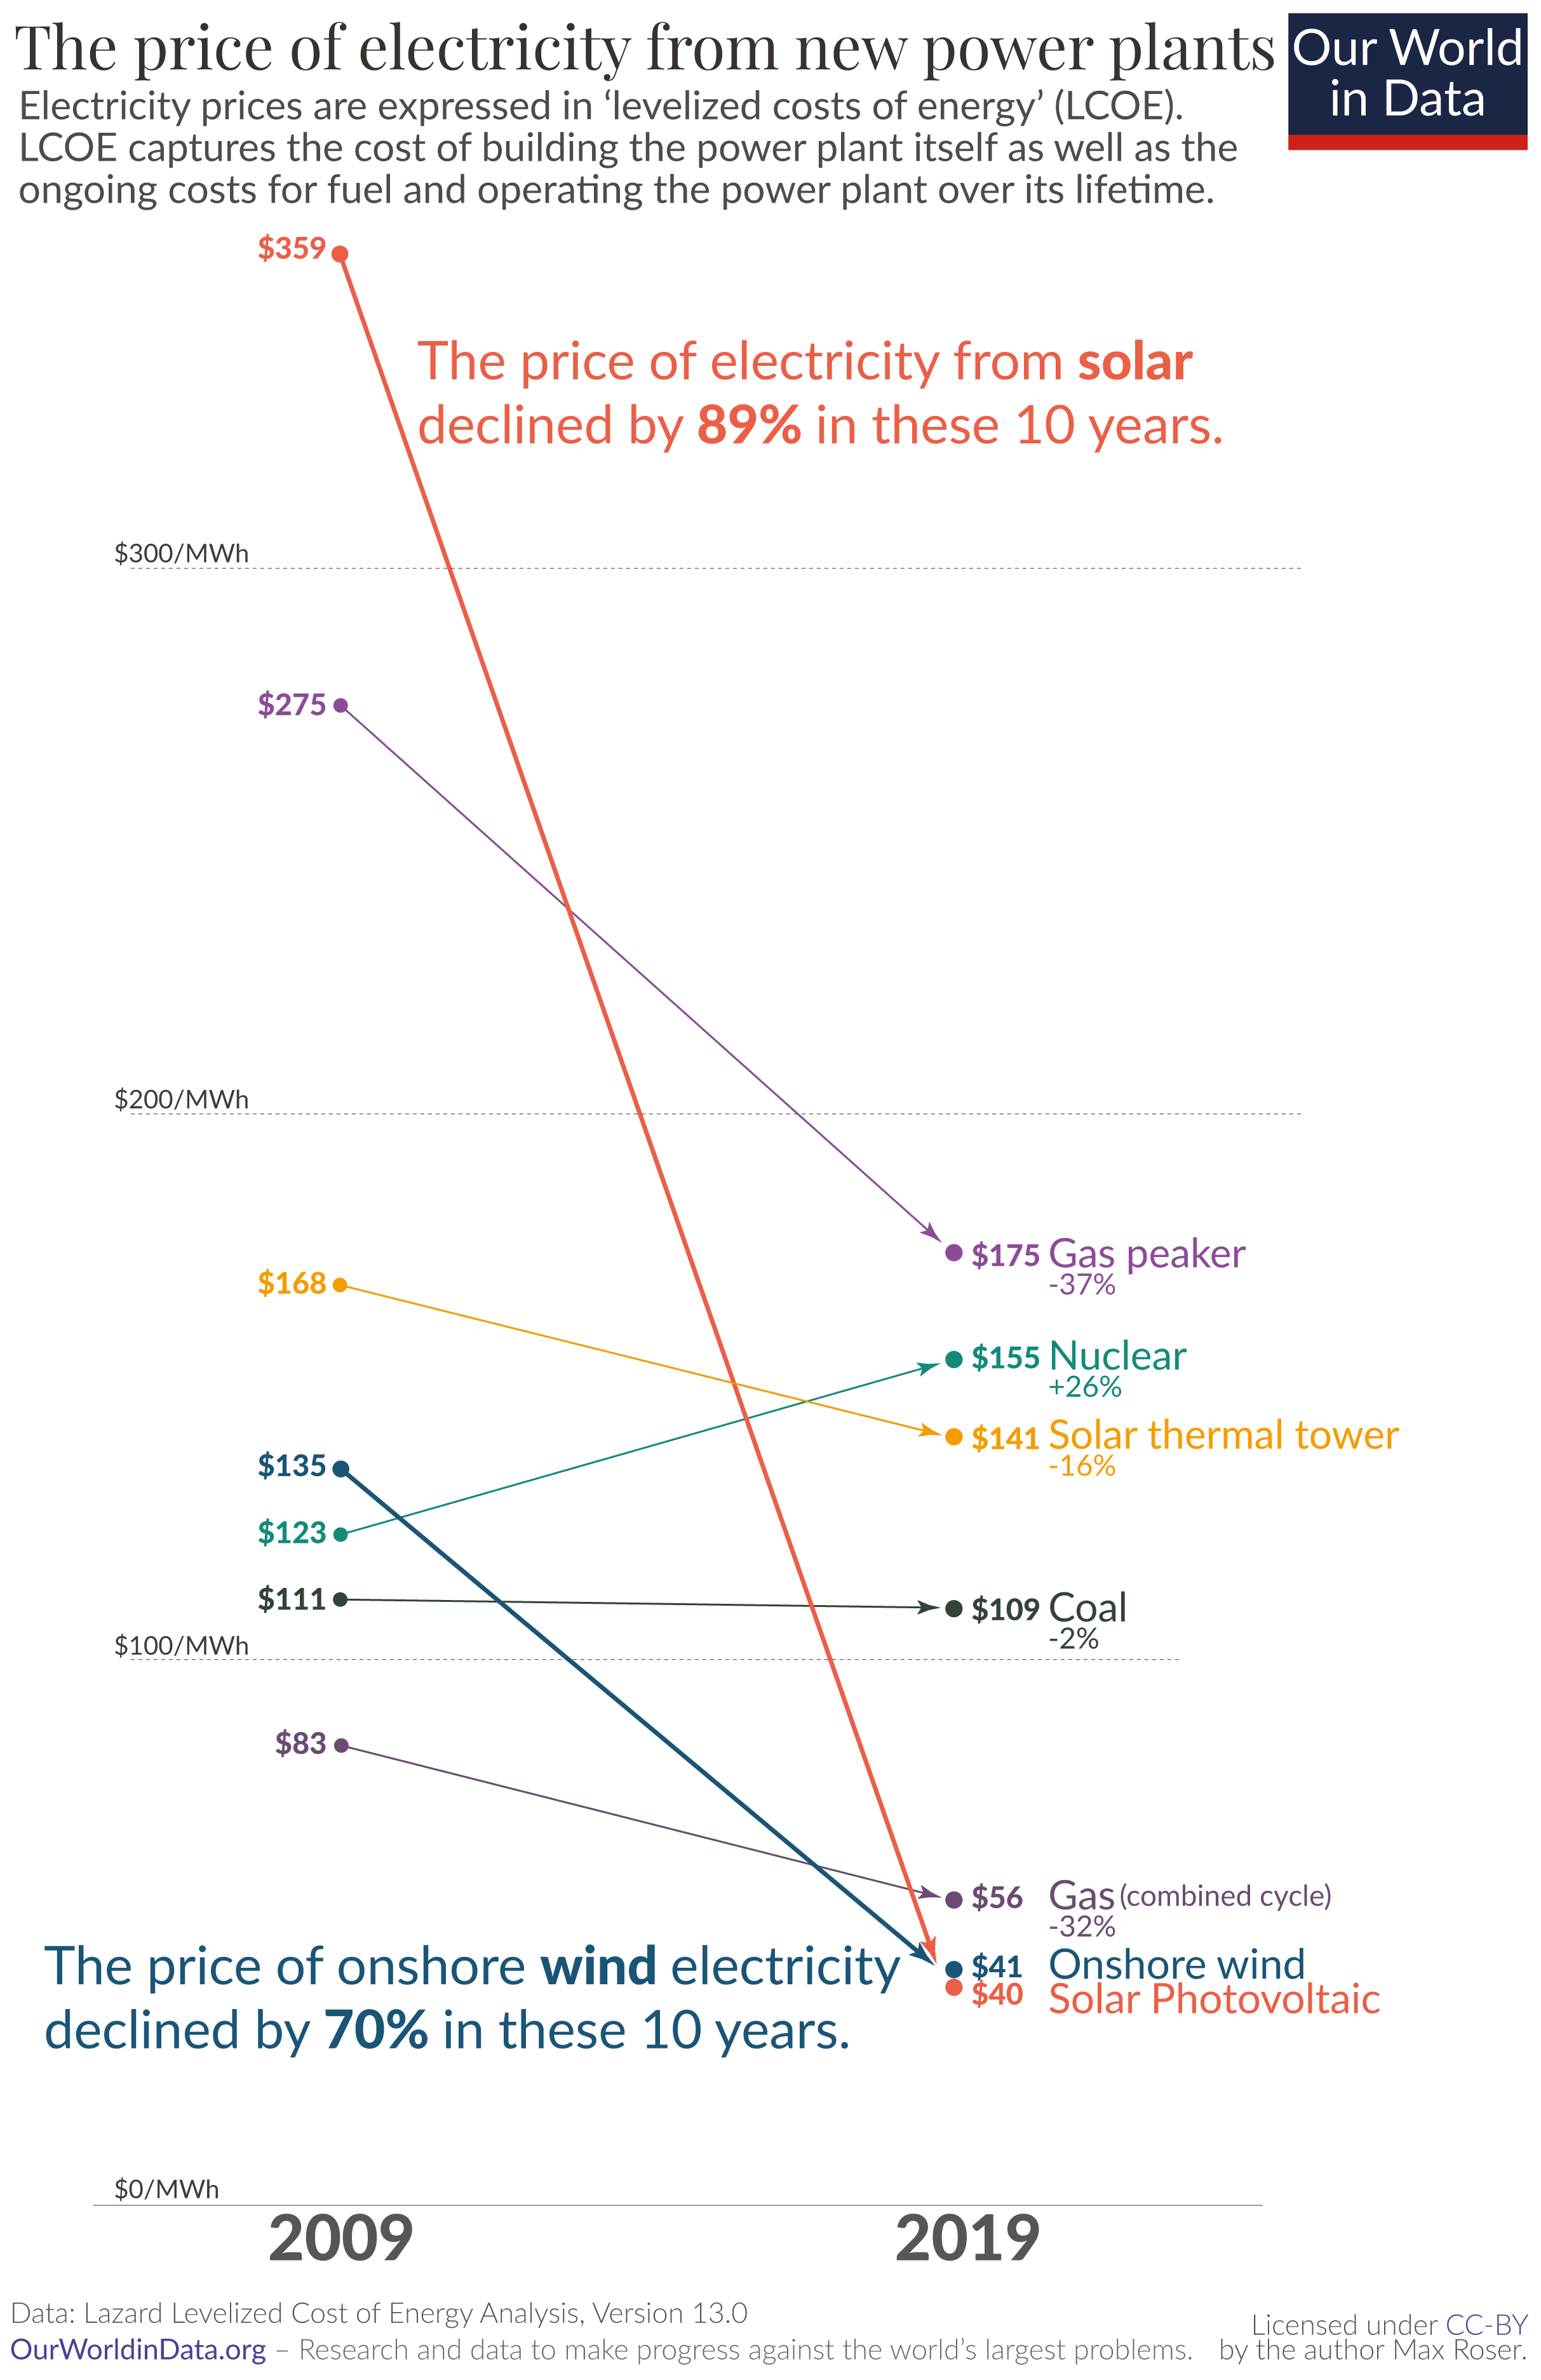
\includegraphics[width=0.8\linewidth]{Energy/ene-costs.png}
%      \caption[Levelised costs of energy for nuclear power]{The levelised costs of energy for nuclear power has been rising in the last 10 years. The costs for renewable energy dropped drastically due to steeply falling learning curves. While prices for wind power declined by 70\,\%, prices of photovoltaics dropped by a factor of 10. Figure taken from Ref.~\cite{OWDcheap}, using data from Ref.~\cite{Lazard}.}
%      \label{fig:ene-costs}
%  \end{figure}

Line 215:

%%% electrons transferring energy 
%%% is this specific to linear accelerators? seems like it

%%% permanent magnet instead of superconducting
%% saves significant energy but reduces flexibility of setup

%%%% https://www.osti.gov/biblio/1412724-cbeta-design-report design report but no numbers? 
%%% https://www.osti.gov/pages/biblio/1650002 PRL article about it

%%%%%

% \begin{to_do}
% More details on energy saving and recuperation for \ACR\ community. See Best Practices \ref{BP:DESY_recycling} and \ref{BP:Nikhef}.\\
% \end{to_do}

FOOD

Line 27:

%~\footnote{The concentration of plant nutrients in natural water systems, sometimes due to fertiliser run-off, giving rise to a decreased capacity to support larger underwater animals.}. 
%Food waste accounts for 6\,\% of total global GHG emissions~\cite{Searchinger2018}, three times the emissions due to aviation~\cite{OWID-Food}.

Line 29:

%Shifting consumption away from animal products to a more plant-based diet significantly reduces the environmental cost of food systems~\cite{PooreNemecek2018, Xu2021}. 

Line 29:

%\fref{carbonopportunity}.  

Line 31:

%Beef, for example, gives rise to twice the emissions per gram of protein of its closest contender on average~\cite{PooreNemecek2018}. 
%Eating less meat, and beef in particular, is among the most significant changes anyone can immediately make in their personal lives on their GHG emissions~\cite{interactive}.  

Line 34:

%In lower-income countries with more limited diets, for instance, small amounts of meat and dairy could provide essential nutrients.


% The food we eat is a deeply personal choice, which is loaded with much cultural and social significance. As such, it is important to acknowledge that changing our food culture will be a gradual process and will not have a `one size fits all' solution.

% However, the excessive amount of meat currently consumed in many countries is neither healthy for the planet, nor for the people consuming it. The conditions under which the meat is produced are unhealthy for animals, as well as the people caring for them, and animal agriculture is possibly a major risk factor for the emergence of new zoonotic diseases~\cite{Jones8399, Espinosa, Morand}.

Line 40:

%, and move towards a more plant-based diet.

Line 44:

%, and inform attendees communicate the reasoning behind these choices with attendees.
% \begin{itemize}
%             \item Orient conference catering towards including more, and more varied, plant-based options, particularly in buffets.
%             \item Clearly label available food items with environmental impact to enable participants to make informed choices.
%             \item Decrease plate size to minimise food waste in buffet settings.
%             \item Provide reusable cutlery and crockery where possible.
%         \end{itemize}

Line 53:

%            \item Use plant-based milk in coffee machines.

Line 82:

%Growth in the food industry is inevitable, and there are limited opportunities to mitigate these costs with improved technology.  Increasing crop yields cannot keep pace with global population growth or dietary shifts due to growing affluence~\cite{Clark370}.
%Growth in the food industry is inevitable, but our environment cannot support business as usual.

Line 84:

%However care must be taken to ensure any shift in food culture is undertaken in a socially and ethically responsible way, taking into consideration 

%Although there is huge range of plant-based substitutes for meat and dairy products, they don't all have the same nutritional content as 


%through over-use of antibiotics in the industry industry also influences the medical outcome of disease outbreaks in humans, through over-use of antibiotics in animal agriculture.  Antibiotics are used to prevent common diseases and enhance growth in livestock.  These are then consumed indirectly by humans as part of their daily diet~\cite{Boeckel2019}.  Antimicrobial resistance~\cite{AMBR2005} and resulting `superbug' infections claimed 1.2 million human lives in 2019, and will be responsible for taking up to an estimated 10 million human lives by 2050, if unchecked~\cite{AMBR2022}. 

%Animal agriculture is potentially a major risk factor for the emergence of new zoonotic diseases~\cite{Jones8399, Espinosa, Morand}. Moreover, as shown in a recent systematic review and meta-analysis of several studies including over 1.4 million adults in total, food choices have a significant impact on the development and progress of coronary diseases~\cite{meat-health}. According to the analysis an intake of 50 grams/day or more of processed meat (bacon, ham, sausages) can increase the risk of coronary diseases by 18\%. Unprocessed meat can raise this risk by 9\%~\cite{meat-health}.

%At present, agriculture, forestry and other land use contribute between 24 to 26\% of GHG emissions, or about one quarter of any individual’s total emissions~\cite{USEPA}.

%%%%%


%%%%%

%In the agriculture sector, 53\% of emissions come from animal agriculture (from land use, livestock and fish farms, and crops for animal feed), 29\% come from crops raised directly for human consumption, and 18\% emissions come from a combination of retail, packaging, transport and food processing. Hence, just at the level of direct emissions, animal agriculture contributes around twice the emissions of plant cultivation for direct human consumption~\cite{OWID-Food, PooreNemecek2018, Xu2021}. Moreover, out of the total habitable land on our planet, around 38.5\% is used for animal agriculture, causing intensive and extensive deforestation (leading to more erratic weather conditions), and habitat destruction. On the other hand, only 11.5\% of the total habitable land is used for human-edible crop production. Despite this breakdown in the use of habitable land, animal-derived foods contribute to only 18\% of global calorie supply and only 37\% of global protein supply~\cite{OWID-Food, PooreNemecek2018, Xu2021}. Organic and local, animal-derived foods often have higher yields of GHG emissions~\cite{Pieper2020}. This is partly because the livestock take longer to grow to an equivalent size.

%Agriculture is responsible for 70\% of global freshwater withdrawals. By 2025, two-thirds of our world’s population may face water shortages~\cite{water-scarcity}. Eutrophication is another important marker for climate change, which has played the part in previous mass extinctions~\cite{eutrophication}. 78\% of the global contribution to eutrophication comes from agriculture~\cite{OWID-Food, PooreNemecek2018, Xu2021}. The impact of agriculture on our biodiversity is also staggering. Of the total land animal biomass distribution on earth, wildlife contributes to only 4--6\%, humans to 36\% and livestock animals to 60\%, causing a massive imbalance~\cite{Bar-On6506} in biodiversity.

Line 93:

%%%%%

%%%%
%\subsection{Health and Inclusivity}



%In addition, a move toward plant-based diets is beneficial from the perspective of cost~\cite{Springmann2021}, as well as inclusivity towards people with religious and other dietary restrictions. In fact, many religions have fasting traditions in which practitioners are expected to abstain from meat/animal products for a time. Moreover, plant-based alternatives offer a viable option for people with certain dietary restrictions, such as lactose intolerance.


%%%%%


%%%%%

Line 126:


%It has also been shown that conference catering could be made entirely vegan, with no decrease in participant satisfaction. Successful examples are YRISW 2019 in Vienna~\cite{YRISW} and WIPC/FEPC 2019 in Montreal~\cite{WIPC} (see \csref{catering_bp}). Conference catering organisers can also present a rough estimate of the carbon dioxide equivalent of every meal, to make consumers aware of their choices~\cite{Pieper2020}. Moreover, traffic light labelling systems, showing red (\ie the topmost of three lights to make the label readable for colourblind people) for high GHG emissions, yellow for numbers in the middle, and green for the lowest emissions (see, \eg Ref.~\cite{Food_Labels_doi:10.1177/0013916521995473}). Allowing registrants to choose their diet/meals in advance also makes it possible to reduce waste.

%Fair-trade and organic coffees are those with the smallest climate impact, having about one third of the carbon footprint of conventional coffee~\cite{lecoq:hal-03069051}, which should motivate to offer more or only products with these certificates. For some of the drinks containing coffee, the highest climate impact comes from the dairy products used. Using non-dairy substitutes reduces the emissions again by a factor of three. %We propose that these alternatives should be offered with coffee at all conferences and in all canteens that want to reduce their climate impact.
%(There may be a preference for different plant-based milks: Ref.~\cite{plantmilk}.)

% Given the scope of the impact of animal agriculture and our immediate need to mitigate anthropogenic emissions, we gathered the following recommendations, based in part on measures already implemented at several universities and other institutes for higher education~\cite{Berlin, EPFL, Cambridge, Goldsmiths}.

% The only and most important individual measure is to reduce the consumption of animal-based food, especially beef, which gives rise to twice the emissions per gram of protein of its nearest contender (see \fref{fig:ghg-per-protein}).

% For cafeterias, canteens and university dining halls we advise (based on measures already implemented at several universities and other institutes for higher education~\cite{Berlin, EPFL, Cambridge, Goldsmiths}) to limit, or even eliminate, animal-derived foods, and to price food products according to their environmental impact wherever possible (with plant-based meals cheaper to purchase than animal-derived ones).

% Further, we advise that the global \ACR\ community be educated about the impact of their food choices on the planet and its people through colloquia, keynote talks at conferences, and optional courses in tertiary education.

% We gathered the following recommendations, which are intended to be taken by all motivated physicists in the sustainable \ACR\
% community to their home institutions, to raise awareness for the people in charge. We grouped the recommendations into three categories: measurements that every physicist can take individually, can consider when organising a conference, or can motivate the respective institute’s canteens and cafeterias to implement.  

% Based on the data in Ref.~\cite{Pieper2020}, conference catering organisers can present for every meal a rough estimate of the carbon dioxide equivalent of the respective meal, to make consumers aware of their choices. This data could be presented together with the usual presentation of ingredients, allergens, etc., on the conference website or printed on the menus. It would be useful to implement a labelling system, so people can judge if the presented numbers are high or low. We suggest labels representing a traffic light, showing red (\ie the topmost of three lights to make the label readable for colourblind people) for high GHG emissions, yellow for numbers in the middle, and green for the lowest emissions (see \eg Ref.~\cite{Food_Labels_doi:10.1177/0013916521995473}). This data could be made public at the registration step so that people are offered the possibility to choose their diet for the conference in advance. This also would make it possible to plan the number of meals in detail and therefore reduce waste.

% It has been proven that it is possible to organise whole conferences with vegan catering, without leading to unsatisfied participants. Successful examples are YRISW 2019 in Vienna~\cite{YRISW} and WIPC/FEPC 2019 in Montreal~\cite{WIPC} (see best practice examples below). Conference organisers should be motivated to search for and try alternative caterers that offer such choices for lunch, dinner, as well as for buffets.

% The measures stated above could also be implemented in canteens and cafeterias of physics institutes. While it requires some additional action, contacting the canteen management about the food choices, labeling and layout can lead to changes that significantly decrease the environmental impact of the whole personnel that uses the respective canteen. The following discussion gives some examples of measurements everyone could ask their respective canteen to consider. Reducing the amount of meat and increasing the amount of vegetables in non-vegetarian dishes already makes a difference, as well as changing the choice of meat.

% As a pioneering step, some universities in the UK, including Cambridge University~\cite{Cambridge} and Goldsmiths University~\cite{Goldsmiths} have banned red meat from their cafeterias.

% Going a step further, it would be a reasonable move to increase the ratio of plant-based meals in canteens. While many canteens already offer vegetarian dishes on a daily basis, we would suggest offering at least one vegan meal every day, taken into account that plant-based food on average has the lowest environmental impact. \begin{comment}since the data shows that this has the strongest climate impact.\end{comment} In many countries, conventional agriculture, including production of meat, is subsidised by the government. This leads to the paradoxical effect that sometimes, vegetarian meals are the most expensive choices. However, we believe that the price charged for purchase of food should reflect its true (unsubsidized) or environmental cost. This would for the most part result in a plant-based option being the cheapest one, and more likely to be selected by price-conscious consumers. Many of traditional and typical meals from all around the world demonstrate how plant-based meals can be healthy, nutritious and still inexpensive. Establishing one meat-free day per week, on which only vegan or at least only vegan and ovo-lacto vegetarian meals\footnote{ovo-lacto referring to the inclusion of eggs and diary} are served, can make people familiar with vegetarian dishes they may have never tried before and remind everyone that it is, at first, an expression of wealth to eat meat every day and, in times of the climate crisis, a luxury we should call into question.

% Fair-trade and organic coffee is the coffee with the smallest climate impact, having about one third of the carbon footprint of conventional coffee~\cite{lecoq:hal-03069051}, which should motivate to offer more or only products with these certificates. For some of the drinks containing coffee, the highest climate impact comes from the dairy products used. Using non-dairy substitutes like almond or oat milk  reduces the emissions again by a factor of three. We propose that these alternatives should be offered with coffee at all conferences and in all canteens that want to reduce their climate impact. (There may be a preference for different plant-based milks: Ref.~\cite{plantmilk})

%To reduce waste during conferences and in canteens, we suggest that the offering of single-serving plastic containers is reduced as much as possible. 
%The use of single-serving plastic containers at conferences and in canteens has a significant impact on waste. Sometimes there are ways to change to reusable containers for take away meals and coffee, like "recup" in Germany~\cite{recup}, which has recently been introduced into the DESY canteen, or offering fully compostable cups in the US in areas where curbside composting is available. If these are not available, offering fewer single-serving containers automatically motivates people to bring their own, most often reusable containers, which reduces waste immediately.

%In some countries (\eg France), disposing of food that is still good for consumption just because the expiration date is reached has already been banned. Instead, the leftover food is mandated to be given to food banks or other charities. Canteens could volunteer to do that for leftover food that is still fit for human consumption.

INTRODUCTION

Line 110:

%The purpose of this document is to improve awareness of the impact that \ACR\ has on the environment, to provide suggestions and encourage immediate action on ways that we, as a community, can play our part in limiting further degradation of the world's climate and ecosystems, as well as to provide impetus for ongoing and collective discussions of how we can make positive changes to our community's work practices, in terms of environmental sustainability and for the issues of social justice from which climate change and environmental degradation cannot be disentangled.
% NIKO: The sentence was too long (it is an enumeration) so I restructured it.

Line 119:

%\scalebox{0.90}{

%\vbox{\begin{mdframed}[]%font=\small]

Line 128:

%two alternative

Line 128:

%Although the exact number should be treated with caution it is clear that the choice to have an additional child is among the highest impact climate actions that can be taken by an individual.

Line 129:

%This is a nuanced and complex issue,

Line 136:

%\end{mdframed}}
%}

TECHNOLOGY

Line 61:

% requirements in form of checklists and required statements in proposals, reviews and reports.

TRAVEL

Line 26:

% \noindent Transport accounted for 16.2\% of global GHG emissions in 2016~\cite{owidsector}.  Most relevant to the \ACR\ community are the sub-categories of passenger aviation (responsible for 1.5\% of global GHG emissions\footnote{Equivalent to 2.5\% of \CdO\ emissions and 3.5\% of ‘effective radiative forcing’ (a closer measure of aviation's impact on global warming)~\cite{Rit20}}), from business travel, and passenger cars (responsible 7\% of global GHG emissions) from commutes to and from the workplace. 
% These figures however belie the significant role that commuting and business travel play in the annual emissions of an \ACR\ researcher (see \fref{fig:Intro-ComparativeEmissions}), for whom frequent trips to experimental sites, conference `tourism', and meetings to undertake international collaborations are common.  Air travel especially is strongly correlated to income level, with the entirety of its emissions derived from only 11\% of the global population, and only 4\% of people taking international flights.  Most \ACR\ scientists likely belong to the top 1\% of the population categorized as frequent flyers~\cite{GOSSLING2020102194}.  Moreover demand for air, rail and car transport is expected to grow strongly with global population, as well as average income.

% Discussions about curbing business travel are highly charged, as active engagement with other members of the scientific community is integral to scientific practice. Moreover, any changes that we make to travel culture have to be considered in the context of other aspects of our working practices, such as hiring decisions, where limits on travel may disproportionately impact early career researchers. At the same time, the reprioritization of business travel and a move toward a greater share of virtual/hybrid formats can have a positive impact both on the climate and on inclusivity.

% Moreover, our current societal infrastructure is set up to facilitate individual travel by car, to the detriment of a large part of the population. \ACR\ institutes, as large employers with a relatively progressive workforce, have the potential to act as instigators of change in this. Making public transport and cycling the preferred options when possible will increase demand for these more sustainable forms of transport and thus encourage cities to improve the infrastructure for them.

Line 42:

%With a global scientific endeavor such as HECAP, it is of course the case that extensive air travel is necessitated by the very nature of our research. We must work on hardware and in collaboration with people in face-to-face meetings, which serve to engage collaborations much better than videoconferencing. This clearly has drawbacks with unequal access to such opportunities that should be remedied by increased access for people with fewer resources, as well as usage of videoconferencing when feasible.

Line 69:

%Short everyday mobility has a major impact on the environment and people.  Commuting via more sustainable means, on foot, or by bicycle or \textcolor{red}{rail}, are the most obvious ways in which to cut down emissions from travel to work.  

Line 74:

%It is unclear if the commuter emissions include only the ca. 10,000 employees, or also ca. 20,000 students, but regardless 

Line 99:

    % DESY takes over 40 Euros of the job ticket offered by the local public transport company&

Line 142:

%country is France. This affects, in particular, the GHG emissions from electricity production: the carbon intensity of the French grid can be a factor of 10 lower than that of other countries, greatly affecting the emission factors of electricity-powered vehicles.

Line 190:



%Participating in conferences and meeting other scientists is an important part of the scientific career path.
% However, the current system, which requires extreme mobility, especially at early career stages, is neither environmentally sustainable nor equitable to all scientists.

% Stringent visa rules make participation in conferences much harder, or well-nigh impossible, if one is from the Global South. Even if one could obtain the visa to travel, the funds to do so are not equally distributed, and travel to conferences, especially those in the desirable locations often chosen for their attraction value, can be prohibitively expensive.

% Beyond this, the need to travel can be extremely complicated and difficult for people with health impairments or care responsibilities. Participating in a conference while parenting small children requires a partner that is willing and able to shoulder their day-to-day care for the duration of the event, a support net that can step in, or the funds to pay for professional care. Even bringing the children along to conferences does not resolve this. Since the burden of childcare in our society is still unequally distributed, this burden falls predominately on female shoulders~\cite{McCarthy}. The same is true for care giving responsibilities for other adults (\eg elderly parents). For scientists with disabilities, travel to foreign cities can pose a variety of challenges, from wheelchair accessibility of the venue, or the after-hours bar, to questions of specialized diets or sufficient rest time.

% Most of these challenges can be circumvented through virtual conference formats, or at least hybrid options that allow for remote talks.
% However, a remote conference requires participants to have a stable internet connection, and devices with which to connect.  Though most scientists can count on fairly stable and decently high speed internet access by this point, this requirement may in some cases still impair participation especially for participants in lower income countries.  One possible remedy for this might be the concept of hub conferences, where the conference has several locations spread globally (\eg Ref.~\cite{Parncutt}).

%%%%%

% \begin{figure}
%     \centering
%     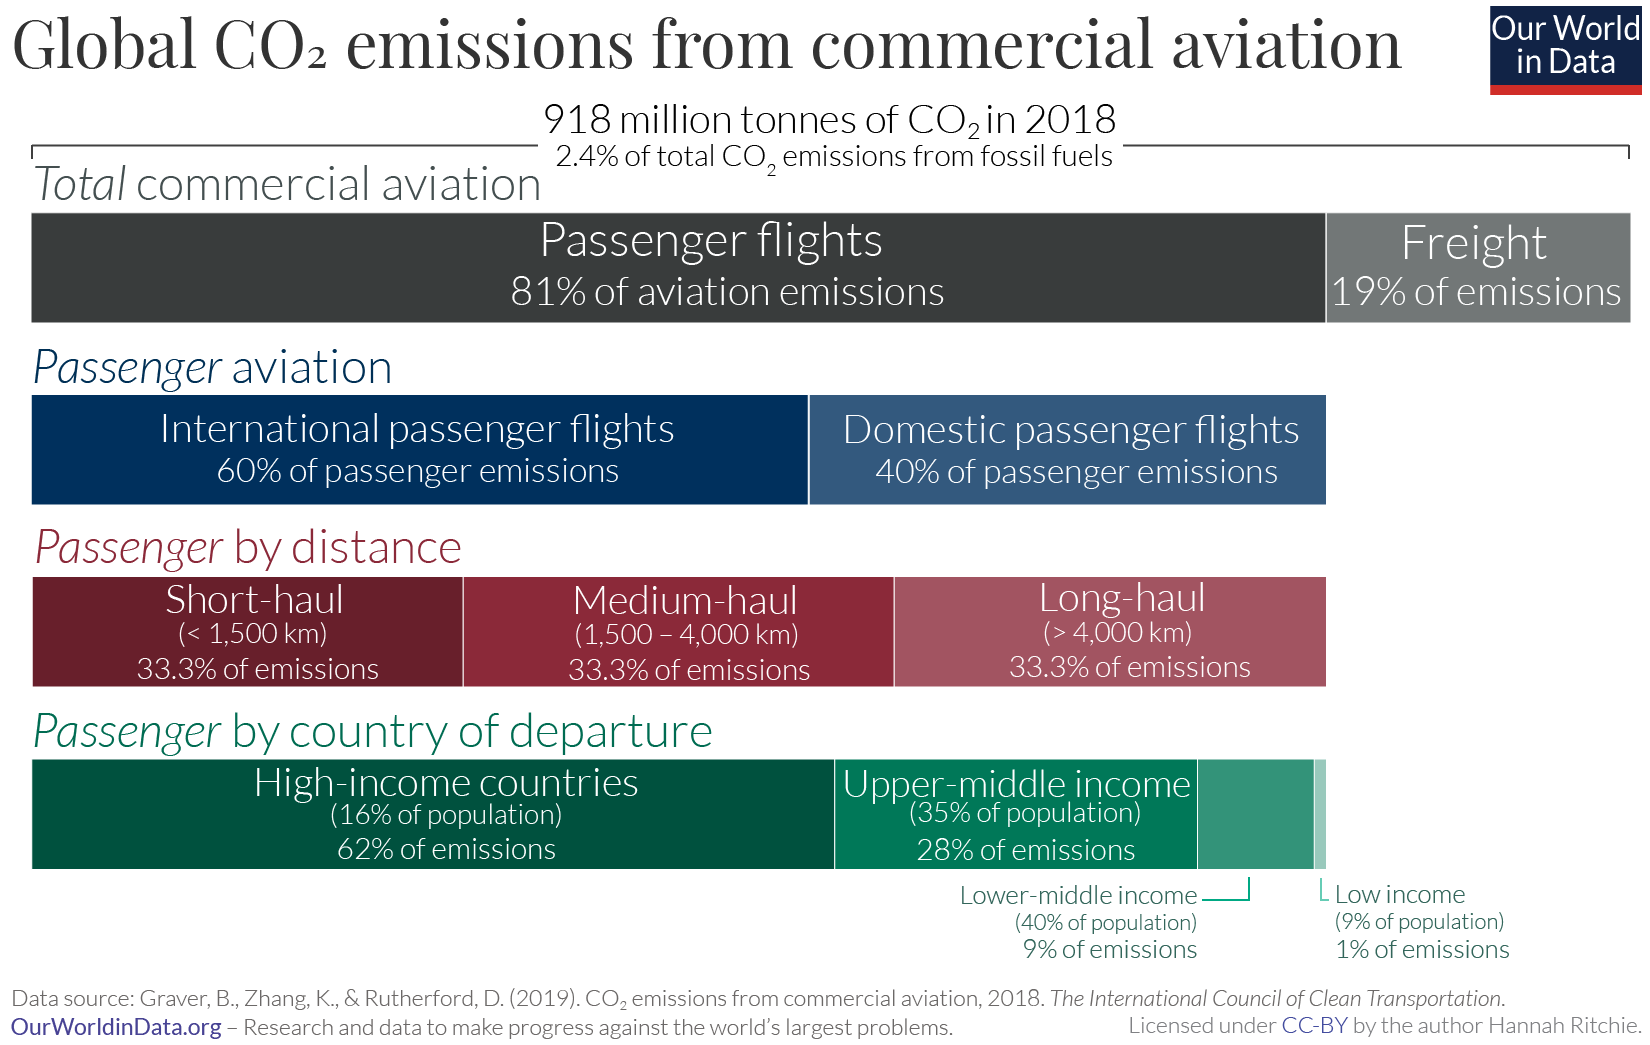
\includegraphics[width=0.85\textwidth]{Sections/Figs/Travel/globalemission_aviation.png}
%     \caption[Global \CdO\ emissions from commercial aviation]%
%         {Global \CdO\ emissions from commercial aviation, reproduced from Our World in Data~\cite{Rit21}, based on data from Ref.~\cite{Graver}.\label{fig:globalemission_aviation}}
% \end{figure}

%%%%%

% \textbf{moved from recommendations - to be included in summary \niko{fix the formatting as well}}
%  These alternative forms are also more inclusive, allowing participation by those who might not otherwise be able to attend due to lack of funding, caregiving responsibilities, institutional policies, or visa (or other political) issues.\\
 
%  Hiring committees should move away from quantifying the worth of a researcher by the amount of travel they have undertaken.\\

Line 324:

%A commonly used Figure of Merit for the power efficiency of computing centres is the so-called Power Usage Effectiveness (PUE), defined as the ratio of the total energy consumption of the facility to the energy consumption of the IT equipment itself. 

Line 367:

%Mandeep Gill: One link on how short-haul flights in Europe are being eliminated: https://www.cntraveler.com/story/how-short-haul-flight-bans-are-transforming-european-travel

Line 371:

%Criticism and discussion of the carbon footprint of conferences is not new~\cite{Spinellis,Ref_AGU, nature_better_confs} and detailed calculations for specific conferences exist alongside reduction scenarios.

Line 423:

%%%%%
% However, this unfortunately can be offset by having the conference be organised in more remote location in a bid to include an active part of the scientific community. Over time this will be compensated, though the timeline for this is of the order of 12 years in total (or in addition to the three in-person ICHEP conference three additional ICHEP conference with a travel profile similar to the Valencia (2014)). It is fair to note, that

%%%%%

% \begin{center}
% \captionsetup{type=table}
% \caption[Number of local participants compared to the average number of participants from that location for the other ICHEP editions]{Number of local participants compared to the average number of participants from that location for the other ICHEP editions (in- and excluding Prague).\niko{ADD REF}}
% \label{tab:localPart}
% \begin{tabular}{@{}p{3.4cm}>{\baselineskip=10pt}p{1.4cm}>{\baselineskip=10pt}p{1.7cm}>{\baselineskip=10pt}p{1.7cm}>{\baselineskip=10pt}p{1.6cm}>{\baselineskip=10pt}p{1.7cm}c@{}}\toprule
% % &
% % % Similarly, one can also consider the fraction of participants for the different travel categories (short journey, short haul, long haul, and super-long haul). This is shown in \fref{fig:DistanceCategories} for the different ICHEP editions, including an average over all ICHEP conferences, except for Melbourne, where over 90 \% of all participants had to travel on a long-haul flight. Generally, the participation is spread relatively evenly over the different categories and surprisingly not so different between the in-person conference average versus the virtual ICHEP conference in Prague. The lower fraction of participants in the short journey category and higher fraction of short haul participants is explained by the fact that there is indeed few other institutes in that range, with participants from within 400 km coming from Dresden, Berlin, G\"ottingen, Munich, Vienna, Bratislava and Cracow. Those from Mainz, Frankfurt, Udine, Slovenian institutes and Budapest being already outside the 400 km range by about $\sim$50 km.

% % The larger amount of local participants is also reflected by looking at how these numbers compared to the average over the participants from that location at the other registered ICHEP conference as reported in \tref{tab:localPart}. Local participants are factor of 3--20 times more likely to participate in a conference, which to some extent should be especially true for young master and PhD students and early career researchers. Note that in this consideration closeby centre with also notably increase participation are not considered (\eg other Spanish or Korean cities).

% % %%%%%

% % \begin{center}
% %     \captionsetup{type=figure}
% %     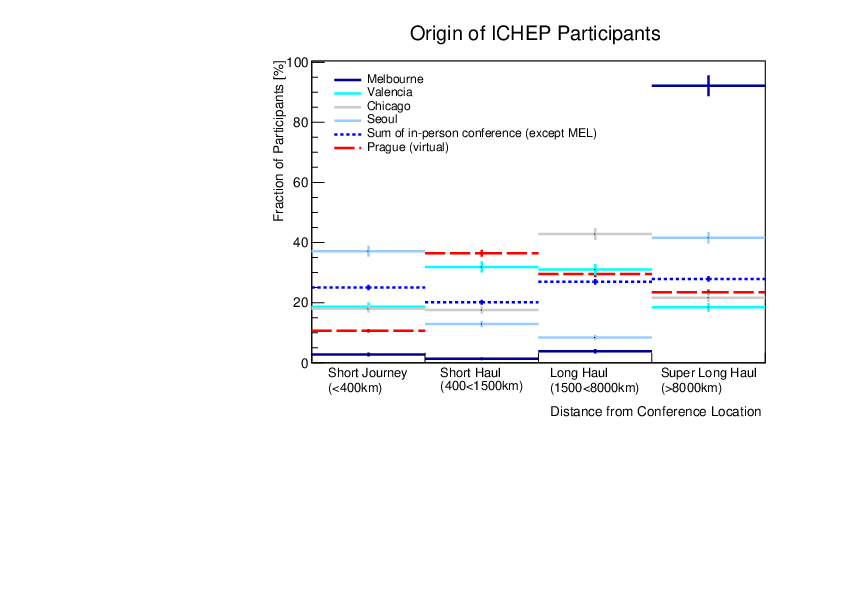
\includegraphics[width=1.\textwidth]{Sections/Figs/Travel/ICHEPParticipants.png}
% %     \caption[Fraction of participants for the different travel categories]%
% %         {Fraction of participants for the different travel categories. Errors are calculated as $\sqrt N$ of the number of participants and propagated accordingly. \niko{INSERT REF}\label{fig:DistanceCategories}}
% % \end{center}

% % %%%%%

% Mel-bourne 2012 & 
% Valencia 2014 &
% Chicago 2016 & 
% Seoul \hspace{0.2cm}2018 &         
% Prague 2020 (virtual) \\ \cmidrule{2-6}
    
% Number of local \hspace{0.6cm}\linebreak participants&
% 21&
% 113     &
% 157    & 
% 375   &  
% 154 &
% \\ \midrule

% Average over other years (including Prague)&
% 4  \linebreak \linebreak (5)    &
% 4 \linebreak\linebreak (12) &
% 30 \linebreak\linebreak (40) &
% 18 \linebreak\linebreak (22) &
% 9 \\ \midrule
        
% How much more likely is local participation (including Prague)&
% 5.3 \linebreak\linebreak (4.2)&
% 28.3 \linebreak\linebreak (9.4)&
% 5.2 \linebreak\linebreak(3.9)&
% 20.8\linebreak \linebreak (17.0)&   
% 17.1 \\  
% \bottomrule
% \end{tabular}
% \end{center}
% %%%%%

Line 424:

%Larger reductions would be only achievable if the local participants would be neglected (or set to the average of the other ICHEP conference). In these cases, the optimal location would move towards Europe with the optimal location using all ICHEP participants 2012--2020 being close to Amsterdam

Line 430:

% Finally, it should be noted that one can look a bit closer at the ICHEP Prague being fully virtual and the impact it has had on underserved communities. ICHEP Prague 2020 counted almost three times as many participants as usual, but did this also correspond to an increase in accessibility? As an indicator, participants where classified according to the human development index (HDI)~\cite{hdiref} of their country of affiliation into four categories (low, medium, high and very high HDI\footnote{Very highly developed countries range from Norway to Malaysia, Kuwait and Serbia, highly developed countries from Trinidad and Tobago and Albania to Egypt and Vietnam. In the medium categories countries ranging from Morocco to Pakistan are included, whilst the low HDI countries include Nigeria down to Chad and Niger. A brief overview over these categories and rankings are available on wikipedia (\url{https://en.wikipedia.org/wiki/List_of_countries_by_Human_Development_Index})}). The share of participants in these categories for each of the ICHEP conferences is shown in \fref{fig:DevelopmentIndex}. Indeed, the ICHEP conference in Prague has the largest proportion of participants from countries with a high or medium human development index\footnote{Virtually no participation from low HDI countries was registered.} of all conferences since 2012 with the participation from very high HDI countries at an all-time low of 82 \%. Generally, for participants from high HDI countries which contributed 11 \%, this seems to follow a general trend of rising participation. To some extend this is true also for participants from medium HDI countries, however for those a relatively large jump from 2.3 \% to 6.1 \% of participants in 2018 and 2020, respectively, is visible.

Line 441:

% The fraction of ICHEP participants depending on their continent of affiliation is shown in \tref{tab:frac_part}. For the last two conference editions also the absolute numbers are shown to demonstrate that the increase in absolute number is even larger. It's equally interesting to have a look at "newcomers" to ICHEP, groups of participants from places that prior to Prague had not been able to participate in the conference. Above a certain number of people from the same institute, the ICHEP participation is an indication of a sustained professional interest and not just of the curiosity of a single random person from a related field. Groups participating for the first time since 2012 in ICHEP came from Lima/Peru (8 participants), Trento/Italy (6 participants), Olomouc/Czech Republic, Casablanca/Morocco, Brasilia/Brazil (5 participants), Tezpur and Jaipur/India, Kuala Lumpur/Malaysia,  Jyväskylä/Finland and Tianjin/China (4 participants each). Some of these new groups come from European institutions and presumably generally have sufficient travel funds, but are perhaps relatively small and by chance did not go to ICHEP in the past few years. However, the majority of new participants comes from lower income countries and are a striking demonstration of how the virtual ICHEP in Prague allowed to increase participation around the globe.

% %%%%%

% \begin{center}
% \ra{1.2}
% \captionsetup{type=table}
% \caption[Fraction of participants per ICHEP]{Fraction of participants per ICHEP with absolute number of participants given in brackets.}
% \label{tab:frac_part}
% \begin{tabular}{@{}r>{\baselineskip=10pt}p{1.7cm}>{\baselineskip=10pt}p{2.cm}>{\baselineskip=10pt}p{1.9cm}>{\baselineskip=10pt}p{1.9cm}>{\baselineskip=10pt}p{1.8cm}c@{}}\toprule
% &ICHEP Melbourne 2012 & 
% ICHEP \hspace{0.2cm} Valencia 2014 &
% ICHEP Chicago 2016 & 
% ICHEP Seoul \hspace{0.2cm} 2018 &         
% ICHEP Prague 2020 (virtual) \\ \cmidrule{2-6}
    
% Europe&
% 52.2\%&
% 66.4\%&
% 34.6\%&
% %382
% 32.4\%&
% %1529
% 53.2\%
% \\

% &
% &
% &
% &
% (382)
% &
% (1529)
% \\ \midrule

% North America&
% 27.6\%&
% 17.6\%&
% 45.4\%&
% %138
% 11.7\%&
% %596
% 20.7\%
% \\ 
% &
% &
% &
% (138)
% &
% (596)
% \\ \midrule
        
% Asia&
% 13.6\%&
% 13.6\%&
% 15.1\%&
% %631
% 53.5\%&
% %591
% 20.6\%
% \\ 
% &
% &
% &
% (631)
% &
% (591)
% \\

% \midrule

% South America&
% 2.4\%&
% 1.3\%&
% 3.6\%&
% %6\hspace{0.4cm} \linebreak
% 0.5\%&
% %101
% 3.5\%
% \\ 
% &
% &
% &
% (6) 
% &
% (101)
% \\ 


% \midrule

% Oceania&
% 4.1\%&
% 0.4\%&
% 0.6\%&
% %14\hspace{0.2cm} \linebreak
% 1.2\%&
% %22\hspace{0.2cm} \linebreak
% 0.8\%
% \\
% &
% &
% &
% (14) 
% &
% (22) 
% \\
% \midrule

% Africa&
% 0.0\%&
% 0.7\%&
% 0.8\%&
% 0.6\%&
% 1.3\%
% \\ 
% &
% &
% &
% (7)&
% (36)
% \\ 

% \bottomrule
% \end{tabular}
% \end{center}

% %%%%%

% A visual representation of the location of the institutions of the ICHEP participants is given in \fref{fig:IchepMaps} (middle panel) for the period from 2012 to 2018. The number of participants is indicated with gray circles for the in-person ICHEP meetings (middle panel) and the meeting held virtually in Prague in 2020 (bottom panel).
% %In greyscale the participants of the different in-person ICHEP conferences are shown, in the bottom particpants of the virtual ICHEP 2020 in Prague are shown.%
% This can be compared to the distribution of HEP institutes around the globe (top panel)\footnote{HEP institutions as listed in the Inspire database are used, which have associated publications after January 1st 2006. Included are also companies and commercial research facilities that have signed publications in recent years as Inspire includes those as institutions on their data base.}. The geographically very asymmetric distribution of HEP researchers is visible, which are located more towards the global North and the more industrialized countries. This explains to some degree Amsterdam as the most optimal conference location. Also visible is the slightly more diverse distribution of participants in the virtual ICHEP conference.

% %%%%%

% \begin{center}
%     \captionsetup{type=figure}
%     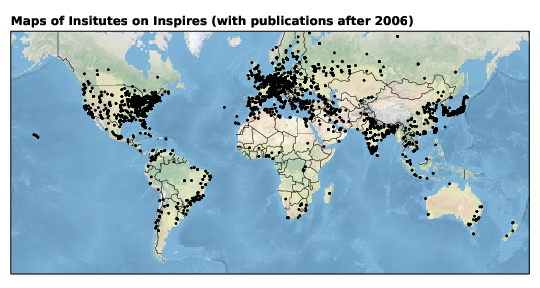
\includegraphics[width=1.\textwidth]{Sections/Figs/Travel/map_inspires.png}
%     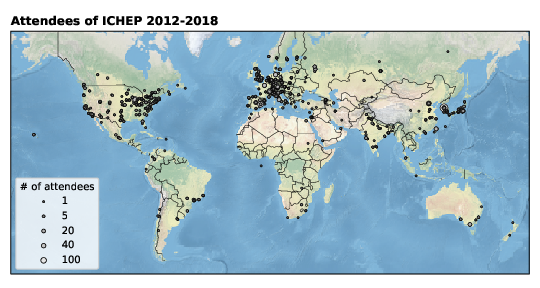
\includegraphics[width=1.\textwidth]{Sections/Figs/Travel/map_COMB.png}
%     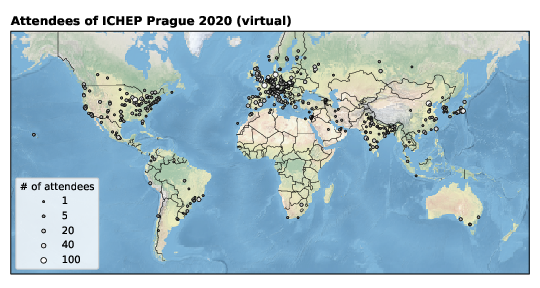
\includegraphics[width=1.\textwidth]{Sections/Figs/Travel/map_PRG.png}
%     \caption[Geographical distribution of ICHEP participants]%
%         {Top: Map of HEP institutions on Inspire with publications after 2006 (one entry per institute, without checking for double countings, though these should overlap and not be visible on the map). Included are also companies and commercial research facilities that have signed publications in recent years as Inspires includes those as institutions on their data base. Middle: Participants of recent ICHEP editions (2012-2018) with a grey scale used for all in-person ICHEP conference with participants of the different years drawn on top of each other. Bottom:  Participants of the virtual ICHEP Prague 2020 edition.\label{fig:IchepMaps}}
% \end{center}

% %%%%%

Line 470:

% \ra{1.05}
% \extrarowheight=\aboverulesep
% \addtolength{\extrarowheight}{\belowrulesep}
% \aboverulesep=0pt
% \belowrulesep=0pt
% \captionsetup{type=table}
% \caption{\label{tab:CERNtravel}Comparison of modes of travel to CERN from different origins.}
% \begin{tabular}{@{\kern\tabcolsep}p{1.8cm}>{\baselineskip=10pt}p{1.5cm}>{\RaggedRight\arraybackslash\baselineskip=15pt}p{3cm}>{\baselineskip=15pt}p{2.0cm}>{\baselineskip=15pt\RaggedRight\arraybackslash}p{11cm}>{\baselineskip=10pt}p{1.1cm}>{\baselineskip=10pt}p{1.5cm}c@{}}
% \toprule
% %& \multicolumn{2}{c}{\ssWW} & \phantom{abc}\\
% \cellcolor{gray!20}Distance &
% \cellcolor{gray!20}Origin &
% \cellcolor{gray!20}Mode of Transport &
% \cellcolor{gray!20}Travel time (one way) &
% \cellcolor{gray!20}Itinerary&
% \cellcolor{gray!20}Price (EUR)&
% \cellcolor{gray!20}Emissions (kg CO$_2$e)
% \\ \cmidrule{1-7}

%%%%%

WASTE

Line 37:

%While the generation of waste products is universal, discussions  specific to the HECAP communities are provided below.

Line 45:

% Minimize printing. Replace workflow elements involving printed materials with appropriate pdf readers/ notetaking apps.

Line 50:

% Reduce or eliminate the distribution of stationery, gifts and printed materials at conferences; minimize the use of plastic.
%     \begin{itemize}
%             % \item Distribute sustainable stationary (recycled paper, sustainably sourced pencils) on a need-only basis, or at a small cost.
%             \item Keep any conference gifts digital \eg e-vouchers/discounts for local restaurants or activities. Distribute sustainable stationary on a need-only basis.
%             \item Make banners, posters and nametags plastic-free and reusable, and share leftover resources with future events.
%             \item Prioritise catering with reusable, washable tableware. For outdoor events with informal catering, use biodegradable tableware with industrial composting of waste.
%             \item Provide alternatives to printed timetables and welcome packs, \eg by making use of  a well-designed conference app (see, \eg Whova\cite{Whova}).
% \end{itemize}

Line 64:

%            , to allow for longer (private) use of the equipment, and reduce the need for new work equipment at every new position.

Line 71:

%            \item Decrease the size of mixed waste bins, and increase the size, availability and prominence of recycle bins.

Line 74:
% \textbf{Reduce or eliminate the distribution of stationery, gifts and printed materials at conferences}; minimize the use of plastic.\\

% %            \item Provide suitable equipment, \ie e-readers, etc, to groups for handwritten notes, reading papers, etc.
%             \item[] Replace printed timetables with a well-designed conference app that has all relevant info.

Line 135:

%Rakhi commenting out until we have official figures/commentary
% \begin{casestudy}[CERN Procurement Emissions]{Emissions due to CERN procurement, 2019}
% \ra{1.05}
% {\centering
% \captionsetup{type=figure}
% \caption[CERN 2019 procurement emissions]{Emissions and cost of CERN procurement, 2019, broken down by source.~\cite{CERNTownHall}}
% \label{fig:CERNProcurement}
% %\begin{figure}
%     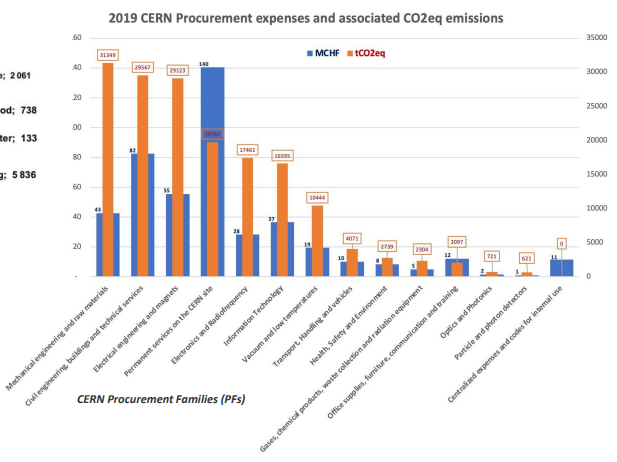
\includegraphics[width=0.9\textwidth]{Waste/CERN-procurement.png}
% %\end{figure}
% }
% \\
% Needs comment.

% \end{casestudy}

Line 163:

% \begin{bestpractice}[\label{case:SupplyChain}Purchasing \& Supply Chains]{Purchasing \& Supply Chains}%
% \noindent There are a number of substances (cobalt for magnets, rare earths for permanent magnets, niobium) that are produced under very difficult conditions, with a high environmental or societal impact.
% If it is impossible to replace them with materials with less impact, a proof of origin from the supplier can be required. (Being aware of the justified criticism on the loopholes that exist there). CERN has stated that it wants to demand more of this from its suppliers.
% In general, purchasing policy can have a major impact as well. Rewarding or prefering suppliers who (can) e.g. deliver a Lifecycle Assessment for their products, even if not required, is a first step. Even better to have purchasing requirements that suppliers have to comply with (responsible sourcing, proof of delivery, no child labor etc), or at least honor these e.g. by factoring in the presence of such proof in price comparisons through a discount. As mostly the funding is public, respective purchsing
% type purchasing regulations need to allow this. Something that can be a question towards funding agencies. CERN says they will first concentrate on suppliers who sell a lot to CERN and where CERN accounts for a large part of the turnover - the ones with the largest impact. ~\cite{Cennini}
% \end{bestpractice}

Line 165:

%\subsubsection{Reduce, Repair, Reuse, (and if all else fails) Recycle}

%\subsubsection{

%RM commenting out until we have more time to flesh this out.
% In order to determine the optimal path for reducing the waste generated by the academic community, one has to first understand the scope of what waste means for different subfields. From there one can identify the sources of waste generation, especially when consumption can be a driver for waste. After making such identifications concrete actions can be defined for reduction of consumption, reduction of waste by re-use and repurposing and finally recycling of the waste generated. Recycling requires treatment, so should be seen as a last resort.  Once these policies have been developed institutions and departments can be approached with  these tailored recommendations, which can then be implemented.

% The waste produced through the activities of HECAP research can be classified into the following three categories, based on the duration of their use, which can help in building strategies for reducing them through policy decisions:
% \begin{itemize}
%     \item Short-term and regular use
%     \begin{itemize}
%         \item Paper: journal articles, official documents, circulars and newsletters, books
%         \item Plastics: stationary, organizational aids (clips, binders, folders)
%         \item Essential consumables: food, chemicals
%         \item Energy: buildings, transportation, computation, running facilities
%     \end{itemize}
%     \item Short-term and irregular use
%     \begin{itemize}
%         \item Conference gifts
%         \item Conference supplies
%         \item Allied footprints of conferences, workshops and meetings
%     \end{itemize}
%     \item Long-term use
%     \begin{itemize}
%         \item Waste generated during the construction, operation and decommissioning/dismantling of infrastructure, \ie experimental facilities.
%         \item Electronic waste: computers, tablets etc.
%         % \item Electrical appliances: coffee machines (a much smaller concern)
%         \item Furniture
%         % \item Constructions with a shorter life cycle, civil engineering for experiments, etc.
%     \end{itemize}
% \end{itemize}

% \begin{to_do}{}
% Further discussion of each of the above, their impact and potential strategies to reduce, reuse, recycle.\\
% \end{to_do}

Line 168:

%After protracted storage at the DESY campus in Hamburg, Germany, 500 heavy concrete blocks originally used for radiation shielding in HERA halls were shreddedshielding blocks

Line 186:

%             \item Keep any conference gifts digital \eg e-vouchers/discounts for local restaurants or activities. Distribute sustainable stationary on a need-only basis.
%             \item Make banners, posters and nametags plastic-free and reusable, and share leftover resources with future events.
%             \item Prioritise catering with reusable, washable tableware. For outdoor events with informal catering, use biodegradable tableware with industrial composting of waste.
%             \item Provide alternatives to printed timetables and welcome packs, \eg by making use of  a well-designed conference app (see, \eg Whova\cite{Whova}).
% \end{itemize}

Appendix A

Line 58:

% \begin{to_do}{}
% Add more details on what emissions contributions are included in each estimate.
% \end{to_do}